%%%%%%%%%%%%%%%%%%%%%%%%%%%%%%%%%%%%%%%%
% Beamer Presentation
% LaTeX Template
% Version 1.0 (10/11/12)
%
% This template has been downloaded from:
% http://www.LaTeXTemplates.com
%
% License:
% CC BY-NC-SA 3.0 (http://creativecommons.org/licenses/by-nc-sa/3.0/)
%
%%%%%%%%%%%%%%%%%%%%%%%%%%%%%%%%%%%%%%%%%

%----------------------------------------------------------------------------------------
%	PACKAGES AND THEMES
%----------------------------------------------------------------------------------------

\documentclass[xcolor=dvipsnames, aspectratio=169]{beamer}

\mode<presentation> {

% The Beamer class comes with a number of default slide themes
% which change the colors and layouts of slides. Below this is a list
% of all the themes, uncomment each in turn to see what they look like.

\usetheme{Madrid} %Hannover
% As well as themes, the Beamer class has a number of color themes
% for any slide theme. Uncomment each of these in turn to see how it
% changes the colors of your current slide theme.
\useoutertheme{infolines} % Alternatively: miniframes, infolines, split
\useinnertheme{circles}
\definecolor{UBCblue}{rgb}{0.04706, 0.13725, 0.26667} % UBC Blue (primary)
\usecolortheme[named=UBCblue]{structure}
}

\usepackage{graphicx} % Allows including images
\usepackage{booktabs} % Allows the use of \toprule, \midrule and \bottomrule in tables
\usepackage{textpos}
\usepackage{caption}
\usepackage[utf8]{inputenc}
\usepackage[brazilian]{babel}
\usepackage{csquotes}
\usepackage{listings}
\setbeamertemplate{caption}[numbered]
\usepackage[style=abnt]{biblatex}
\addbibresource{bibliography.bib}
\PassOptionsToPackage{useregional}{datetime2}
\usepackage{xcolor}


\definecolor{codegreen}{rgb}{0,0.6,0}
\definecolor{codegray}{rgb}{0.5,0.5,0.5}
\definecolor{codepurple}{rgb}{0.58,0,0.82}
\definecolor{backcolour}{rgb}{0.95,0.95,0.92}
\definecolor{string-color}{rgb}{0.3333, 0.5254, 0.345}

\lstdefinestyle{mystyle}{
    backgroundcolor=\color{backcolour},   
    commentstyle=\color{codegreen},
    keywordstyle=\color{string-color},
    keywordstyle=[2]{\color{codepurple}},
    keywordstyle=[3]{\color{magenta}},
    numberstyle=\tiny\color{codegray},
    stringstyle=\color{codepurple},
    basicstyle=\ttfamily\footnotesize,
    breakatwhitespace=false,         
    breaklines=true,                 
    captionpos=b,                    
    keepspaces=true,                 
    numbers=left,                    
    numbersep=5pt,                  
    showspaces=false,                
    showstringspaces=false,
    showtabs=false,                  
    tabsize=2,
    otherkeywords = {tf, Sequential, SimpleRNN, Dense, GRU, LSTM},
    morekeywords = [3]{keras},
}

\lstset{style=mystyle}
\newcommand{\source}[1]{\vspace{-20pt} \caption*{ Fonte: {#1}} }
\usepackage{copyrightbox}


\makeatletter
% \beamer@nav@subsectionstyle{hide/hide/hide}
\addtobeamertemplate{sidebar left}{%
\hspace{0.5cm}
\includegraphics[width=0.9cm, keepaspectratio]{figures/_brasao_ufsm_cor.png}
% \hspace{2.3cm}
\includegraphics[width=0.8cm, keepaspectratio]{figures/brasao_ctism.png}
% \hspace{2.3cm}\includegraphics[width=1.5cm, keepaspectratio]{_logosbc.png}
% \hspace{2.3cm}\includegraphics[width=1.5cm, keepaspectratio]{_logoERRC.png}%
}{}


\setbeamertemplate{footline}
{
	\leavevmode%
	\hbox{%
	    %\hspace{0.25cm}
\includegraphics[width=2cm, keepaspectratio]{figures/brasao_ufsm_cor.png}
		\begin{beamercolorbox}[wd=.333333\paperwidth,ht=2.25ex,dp=1ex,right]{date in head/foot}%
			\usebeamerfont{date in head/foot}\insertshortdate{}\hspace*{2em}
			\insertframenumber{} / \inserttotalframenumber\hspace*{2ex} 
		\end{beamercolorbox}}%
		%\vskip0pt%
	}
\makeatother

%----------------------------------------------------------------------------------------
%	TITLE PAGE
%----------------------------------------------------------------------------------------

\title[]{Microwave Radar and Millimiter-Wave Radar} % The short title appears at the bottom of every slide, the full title is only on the title page

\author[]{Fábio Demo da Rosa} % Your name
%\includegraphics[]{logositeredes.png}
\institute[UFSM] % Your institution as it will appear on the bottom of every slide, may be shorthand to save space
{
Universidade Federal de Santa Maria \\ % Your institution for the title page
Pós-Graduação em Ciência da Computação \\
Disciplina de Robótica Móvel\\
\medskip
\textit{faberdemo@gmail.com} % Your email address
}
\date{25 de Agosto de 2023} % Date, can be changed to a custom date
\newcounter{saveenumi}
\newcommand{\seti}{\setcounter{saveenumi}{\value{enumi}}}
\newcommand{\conti}{\setcounter{enumi}{\value{saveenumi}}}

\resetcounteronoverlays{saveenumi}


\begin{document}

\begin{frame}
\titlepage % Print the title page as the first slide
\end{frame}

\begin{frame}
\frametitle{Visão Geral} %\includegraphics[]{logositeredes.png}} % Table of contents slide, comment this block out to remove it
\tableofcontents % Throughout your presentation, if you choose to use \section{} and \subsection{} commands, these will automatically be printed on this slide as an overview of your presentation
\end{frame}

%----------------------------------------------------------------------------------------
%	PRESENTATION SLIDES
%----------------------------------------------------------------------------------------

%------------------------------------------------
\section[Microwave Radar]{Microwave Radar} 
%------------------------------------------------
\begin{frame}[allowframebreaks, fragile]
\frametitle{Microwave Radar}
	\begin{itemize}
		\item A porção do espectro eletromagnético considerada uma frequência útil para radares práticos é entre 3 e 100 GHz;
		\item A maioria dos radares convencionais operam nas bandas L, S C ou X;
		\item A lista de letras (Figura) foi adotada como medida de segurança durante a Segunda Guerra Mundial, e foi mantida por conveniência;
		
		\begin{figure}
            \centering
            \copyrightbox[b]{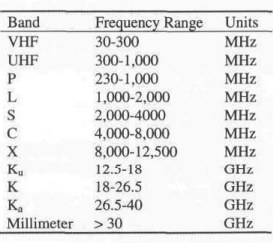
\includegraphics[scale=0.45]{figures/1_MR_frequency_bands.png}}%
            {Fonte: \cite{everett1995sensors}}
            \caption{Bandas de frequência designadas para frequências de radares (IEEE Standard 521-1976).}
            \label{fig:curva_de_freq}
        \end{figure}

    \newpage
    \item O radar utiliza radiação de micro-ondas para detetar o alcance, a distância e outras características dos dispositivos de deteção, além de aplicações móveis de banda larga \cite{Agarwal_2021}.
    \item O cálculo de distância é obtido por métodos TOF, CW phase Detection ou CW Frequency Modulation;
    \item \textit{Pulsed Systems} pode detectar alvos em distâncias de até centenas de quilômetros, dependendo na medida do tempo de propagação de uma onda propagada na velocidade da luz.
    \item \textit{Near-field measurements} (menos de 100 km) são mais difíceis para esse tipo de sistema;
    \begin{itemize}
        \item Pois sinais nítidos de curta duração são difíceis de se gerar para distâncias inferiores a um pé.
    \end{itemize} 
    \item Radares de onda contínua (CW) são efetivos para curtas distâncias.
    \begin{itemize}
        \item Pois \textit{phase-detection} ou \textit{frequency-shift} não são dependentes na velocidade da onda;
        \item Além de também serem adequadas para medir a velocidade de objetos em movimento por meio de métodos Doppler.
    \end{itemize}
	\end{itemize}
	
\end{frame}


    \subsection[Aplicações]{Aplicações} 
    \begin{frame}[allowframebreaks, fragile]
    \frametitle{Aplicações}
        \begin{itemize}
            \item Amplamente empregados em:
            \begin{itemize}
                \item Vigilância militar e comercial;
                \item Aplicações de navegação;
                \item Detecção de curto alcance (radar de alerta de controle para aeronaves);
                \item Indicadores de nível de tanques;
                \item Controles de tráfego e de velocidade de veículos;
                \item Sensores de movimento e detectores de presença;
                \item Forno micro-ondas.
            \end{itemize}
            \item As micro-ondas são ideais para detecção de logo alcance, porque a resolução é geralmente boa, a atenuação dos feixes na atmosfera é minima;
            \begin{itemize}
                \item Operando em distâncias de alguns metros a algumas centenas de metros.
            \end{itemize}
            \item Radar de micro-ondas do espectro têm menos aplicabilidade às necessidades de prevenção de colisões de curto alcance de uma plataforma robótica móvel.
        \end{itemize}
    \end{frame}

    \subsection[Fatores de Performance]{Fatores de Performance} 
    \begin{frame}[allowframebreaks, fragile]
    \frametitle{Fatores de Performance}
        \begin{itemize}
            \item Aumentar o diâmetro do refletor resulta em uma melhoria na capacidade de alcance devido ao feixe de saída estar focalizado, e quanto mais larga a área da antena, maior a superfície de recepção/transmissão.
            \begin{itemize}
                \item Porém isso pode apresentar desvantagens em manipular um sistema mecânico com alta carga inercial.
            \end{itemize}
            		
		\begin{figure}
            \centering
            \copyrightbox[b]{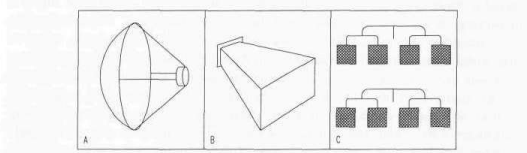
\includegraphics[scale=0.7]{figures/4_MR_commom_configuration.png}}%
            {Fonte: \cite{everett1995sensors}}
            \caption{Configurações comuns das antenas de micro-ondas incluem: (A) prato refletor com ponto focal. (B) Antena tipo corneta. (C) matrizes bidimensionais de microfita}
            \label{fig:MR_commom_config}
        \end{figure}
        
            \item Muitas aplicações comerciais de curto alcance usam a antena tipo corneta para não lidar com os problemas citados;
            \item As configurações de antenas \textit{phased array} (Figura 9-9C) apresentam um arranjo de múltiplas antenas pequenas separadas por distâncias de alguns comprimentos de onda;
            \item Um dos fatores que atrapalha a performance significativamente é a atenuação atmosférica;
            \begin{itemize}
                \item Chuva e neve podem causar atenuação significativa em sinais acima de 2 GHz;
                \item Interferência multipercurso do solo; 
                \item Refletividade e diretividade da superfície alvo;
                \item Cobertura natural, como neve ou folhagem.
            \end{itemize}
        \end{itemize}
    \end{frame}

%------------------------------------------------
\section[Millimeter-Wave Radar]{Millimeter-Wave Radar} 
%------------------------------------------------
\begin{frame}[allowframebreaks, fragile]
\frametitle{Millimeter-Wave Radar}
	\begin{itemize}
		\item As ondas milimétricas constituem aquela porção do espectro eletromagnético com comprimentos de 30 a 300 GHz \cite{everett1995sensors};
		\begin{itemize}
            \item Entre micro-ondas e electro-ótico.
        \end{itemize} 
		\item Têm capacidade de alcance significativamente menor do que os sistemas que usam micro-ondas;
		\item \begin{itemize}
            \item Principalmente devido à atenuação atmosférica e retroespalhamento (considerando principalmente em radares de busca e de sistemas aéreos).
        \end{itemize}
		\item Para aplicações de curto alcance, o desempenho das ondas milimétricas é na verdade superior ao das microondas sob condições climáticas adversas;
		\begin{itemize}
            \item Devido ao comprimento de ondas mais curto, produzem medições de alcance e Doppler mais precisas;
            \item A relação entre o comprimento de onda e o tamanho do alvo melhora para frequências mais
            altas, permitindo uma melhor detecção de pequenos objetos, como postes, fios, árvores e sinais
            de trânsito
        \end{itemize}
        \item As altas frequências Doppler proporcionam boa detecção de alvos em movimento lento. Os baixos requisitos de energia
        de comprimentos de onda mais curtos são atraentes para aplicações robóticas. 
        \item Além disso, comprimentos de onda mais curtos traduzem-se em componentes menores, o que leva a tamanho e
        peso reduzidos; 
        \item As desvantagens são que a atenuação atmosférica aumenta e os tamanhos
        menores da antena levam à redução da sensibilidade do receptor.
	\end{itemize}
\end{frame}


    \subsection[Introdução]{Aplicações} 
    \begin{frame}[allowframebreaks, fragile]
    \frametitle{Aplicações}
        \begin{itemize}
            \item Os usos mais comuns incluem:
            \begin{itemize}
                \item Sensoriamento ambiental;
                \item Radar de imagem com alta resolução;
                \item Espectroscopia;
                \item Equipamentos de telêmetro;
                \item Frenagem de automóveis.
            \end{itemize}
            \item Embora, o uso mais comum seja rastreamento e designação de alvos com fins militares \cite{everett1995sensors}.
            \item A estreita largura de feixe das transmissões de ondas milimétricas é altamente
            imune a problemas de reflexão do sol.
            \begin{itemize}
                \item Radares de busca de micro-ondas de longo alcance
                e feixe largo para aquisição inicial e depois mudando para um radar de rastreamento
                milimétrico para controle do sistema de armas
            \end{itemize}
            \item Sistemas de ondas milimétricas de curto alcance e baixa potência parecem ser
            adequados para evitar colisões e necessidades de navegação de um robô móvel
            externos.
            \item a capacidade de usar antenas menores é uma característica
            dominante que influencia a seleção de ondas milimétricas em micro-ondas. 
            \begin{itemize}
                \item As três plataformas mais diretamente afetadas: satélites, mísseis e mini-RPVs (\textit{Remotely Piloted Vehicles}).
            \end{itemize}
        \end{itemize}
    \end{frame}

    \subsection[Introdução]{Fatores de Performance} 
    \begin{frame}[allowframebreaks, fragile]
    \frametitle{Fatores de Performance}
        \begin{itemize}
            \item O
        \end{itemize}
    \end{frame}

%------------------------------------------------
\section[Considerações Finais]{Considerações Finais} 
%------------------------------------------------
\begin{frame}[allowframebreaks, fragile]
\frametitle{Considerações Finais}
	\begin{itemize}
		\item O sensoriamento baseado em radares de micro-ondas e ondas milimétricas é um tópico de pesquisa importante \cite{cardillo_2023};
        \item Considerando esses ambos radares, os modos de operação e as tecnologias mais populares são:
        \begin{itemize}
            \item Ondas contínuas moduladas em frequência (FMCW); 
            \item Chaveamento por mudança de frequência (FSK), 
            \item Interferometria; 
            \item Doppler;
            \item Banda ultralarga (UWB); 
            \item Formação de feixe digital/RF;
            \item Múltiplas entradas e múltiplas saídas (MIMO);
            \item Radar de abertura sintética (SAR).
        \end{itemize}

        \begin{figure}
            \centering
            \copyrightbox[b]{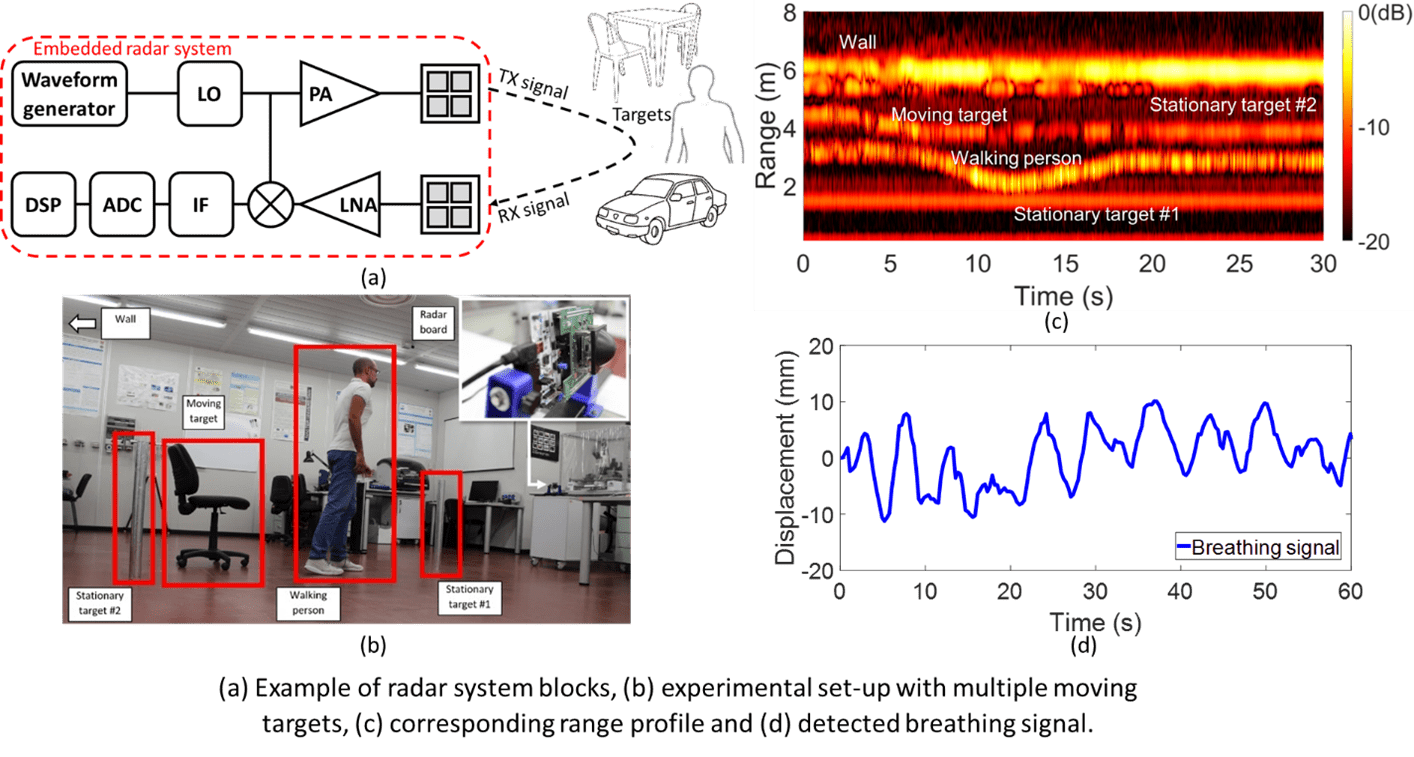
\includegraphics[scale=0.25]{figures/5_tc_microwave.png}}%
            {Fonte: \cite{cardillo_2023}}
            \label{fig:tc_microwave}
        \end{figure}

	\end{itemize}
\end{frame}

%------------------------------------------------
%\section*{Referências}
%------------------------------------------------

\begin{frame}
    % \nocite{*}
    \printbibliography
\end{frame}


\begin{frame}
\titlepage % Print the title page as the first slide
\end{frame}

\end{document}